\begin{figure}[b]
\centering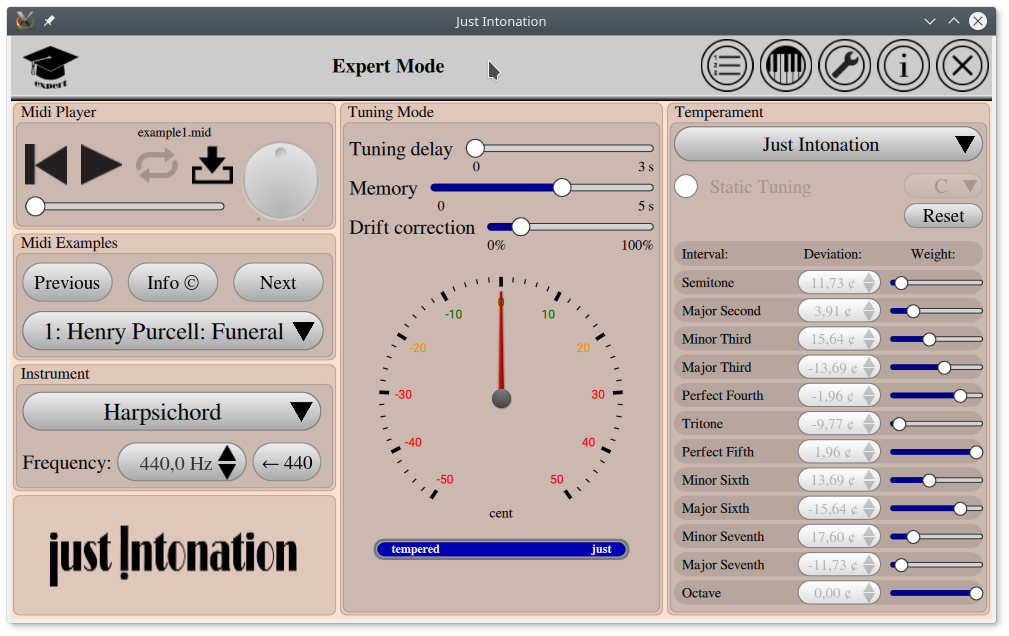
\includegraphics[width=100mm]{screenshot}
\caption{\label{JIapp}
Snapshot of the application \textit{Just Intonation} in the expert mode.
}
\end{figure}

In order to demonstrate the tuning method discussed in this paper, we initiated an open-source project called~\textit{\cite{JustIntonation}} (the present paper refers to version 1.3.2).  This software allows the user to hear and play music with and without adaptive tuning.  Audio examples, a short video and download links for various platforms are available on our website \href{http://www.just-intonation.org}{\texttt{www.just-intonation.org}}.

The application  has been designed as an educational application rather than a professional tool for producing music. It provides a \textit{simple mode} for getting started as well as an \textit{expert mode} for more sophisticated experiments (see screenshot in Fig.~\ref{JIapp}).

\textit{Just Intonation} is a multi-platform application for desktop computers and mobile devices written in C++  based on Qt\texttrademark\footnote{Qt\texttrademark ~is a cross-platform application framework licensed under LGPL that is used for developing application software, see \href{https://www.qt.io/}{\tt www.qt.io/}}. As sketched in Fig.~\ref{appstructure}, it contains various submodules which partially run in different threads and communicate with each other via Qt signals. MIDI messages generated by an integrated player or an external device are sent to the tuning module and to the sound-generated modules. Depending on the MIDI data the tuning module continually computes the vector $\vec\lambda^\OPT$ according to the formulas given above and and emits the calculated pitches via Qt signals to the audio modules. The application includes an built-in microtonal sampler which can play triangular waves as well as realistic samples recorded by the authors (piano, organ, and harpsichord). As the application is designed primarily for educational purposes, there is no particular emphasis on low-latency audio. 

Alternatively, it is possible to connect an external MIDI device which is capable of processing 'pitch-bends'. Normally the MIDI pitch-bend command modifies the frequencies of all depressed keys uniformly. In order to circumvent this restriction, the MIDI output module remaps the incoming MIDI stream to 15 different channels, tuning each of them individually via pitch-bend. Note that this restricts the output to a 15-voice polyphony of a single instrument. It should be mentioned at this point that the MIDI standard has recently been extended. This new standard, called ``MIDI Polyphonic Expression''~\cite{MPE}, overcomes the aforementioned limitations and allows for a direct microtonal control of the individual pitches. 

%------------------------------------
\begin{figure}
\centering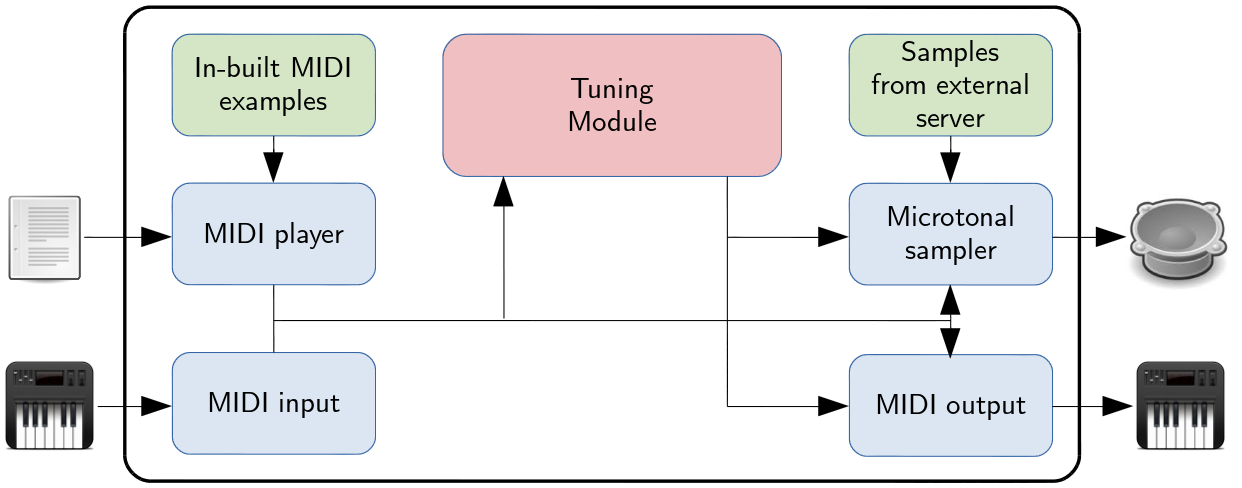
\includegraphics[width=130mm]{appstructure}
\caption{\label{appstructure}
Basic structure of the application and its modules.}
\end{figure}
%------------------------------------

The main module of interest is the tuning module. This module runs entirely in a separate event loop of an independent thread and communicates with the application via Qt signals, ensuring thread safety. Its internal structure is shown in Fig.~\ref{tunermodule}. Its main functionality is 
%
\begin{itemize}
\item receiving MIDI signals and sending tuning signals,
\item emulating the intensity $I(t)$ as well as the memory $M(t)$ for each key of the keyboard,
\item keeping track of the status of the keys (including on/off, volume and basic envelope) in an array of type $\tt KeyData$,
\item executing the {\tt TunerAlgorithm} every 20ms or upon incoming MIDI events, and 
\item managing the pitch drift compensation.
\end{itemize}

For further technical details and code excerpts the interested reader is referred to Appendix~B.

%------------------------------------
\begin{figure}
\centering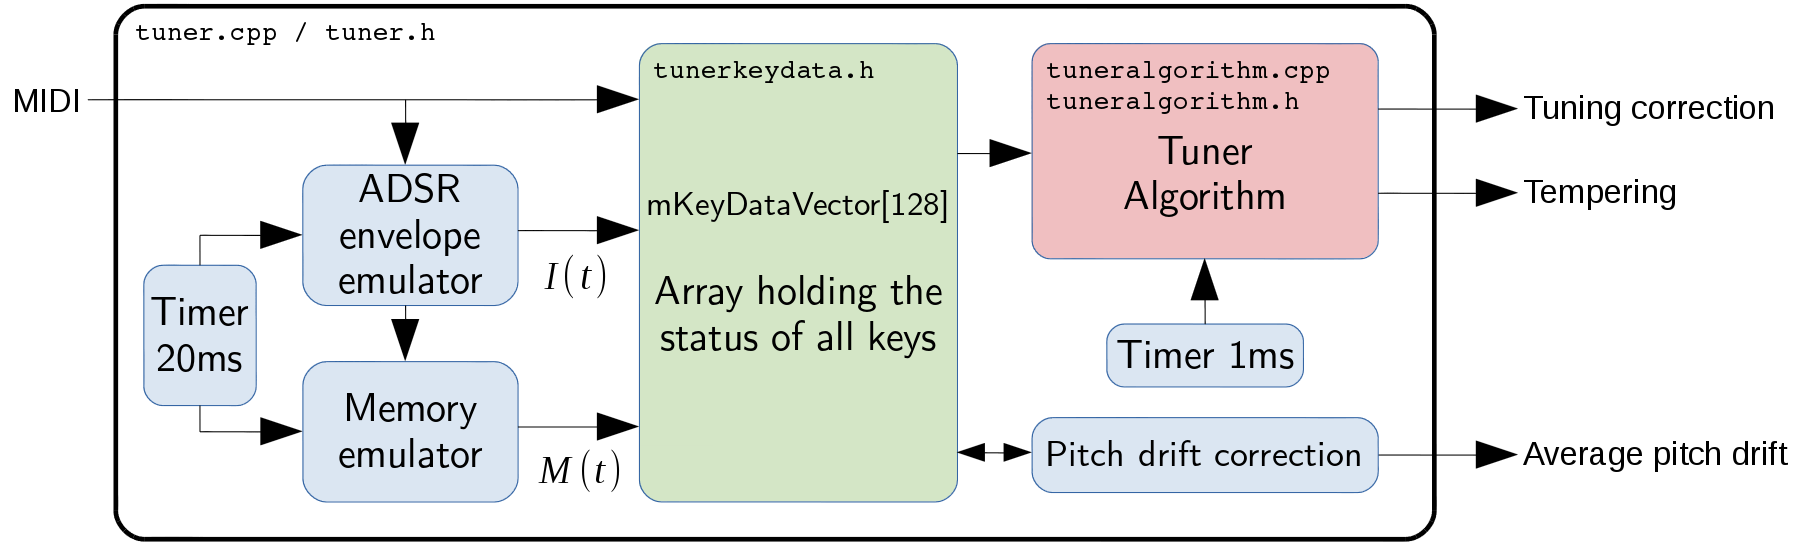
\includegraphics[width=150mm]{tunermodule}
\caption{\label{tunermodule}
Internal structure of the tuner module.}
\end{figure}
%------------------------------------

